\documentclass[11pt]{article}
\usepackage[hmargin=1in,vmargin=1in]{geometry}
\usepackage{xcolor}
\usepackage{pgf}
\usepackage{tikz}
\usetikzlibrary{shapes, arrows}
\usepackage{amsmath,amssymb,amsfonts,url,sectsty,framed,tcolorbox,framed}
\newcommand{\pf}{{\bf Proof: }}
\newtheorem{theorem}{Theorem}
\newtheorem{lemma}{Lemma}
\newtheorem{proposition}{Proposition}
\newtheorem{definition}{Definition}
\newtheorem{remark}{Remark}
\newcommand{\qed}{\hfill \rule{2mm}{2mm}}

\begin{document}
%%%%%%%%%%%%%%%%%%%%%%%%%%%%%%%%%%%%%%%%%%%%%%%%%%%%%%%%%%%%%%%%%%%%%%%%%%%%%%%%%%%%%%%%%%%%%%%
\noindent
\rule{\textwidth}{1pt}
\begin{center}
{\bf [CS304] Introduction to Cryptography and Network Security}
\end{center}
Course Instructor: Dr. Dibyendu Roy \hfill Winter 2023-2024\\
Scribed by: Sanidhya Kumar (202151138) \hfill Lecture (Week 10)
\\
\rule{\textwidth}{1pt}
%%%%%%%%%%%%%%%%%%%%%%%%%%%%%%%%%%%%%%%%%%%%%%%%%%%%%%%%%%%%%%%%%%%%%%%%%%%%%%%%%%%%%%%%%%%%%%%

\section{Modular Equations}
We'll explore solving systems of linear equations to find \( x \) in the form:
\begin{center}
    \( a \cdot x \equiv b \mod m \)    (Eq.1)
\end{center}
To begin, let's express Eq.1 as:
\begin{center}
    \( a \cdot x - m \cdot y = b \)     (Eq.2)
\end{center}
where \( y \) is an integer. Utilizing Bezout's Identity:
\begin{center}
    \( a \cdot x_0 + m \cdot y_0 = \gcd(a, m) \)    (Eq.3)
\end{center}
where \( x_0 \) and \( y_0 \) can be determined using the Extended Euclidean Algorithm.

Eq.2 is solvable if and only if \( \gcd(a, m) \) divides \( b \). Assuming \( \gcd(a, m) \) divides \( b \), we have:
\begin{center}
    \( t \cdot \gcd(a, m) = b \)
\end{center}
By multiplying Eq.3 by \( t \), we get:
\begin{center}
    \( a \cdot (t \cdot x_0) + m \cdot (t\cdot y_0) = t \cdot \gcd(a, m) \implies a \cdot  X_0 + m \cdot Y_0 = b \)
\end{center}

Hence, given an equation to solve, we first verify if \( \gcd(a, m) \) divides \( b \). If so, a solution exists. Then, we find \( x_0 \) and \( y_0 \) using the Extended Euclidean Algorithm and multiply them by \( t = \frac{b}{\gcd(a, m)} \) to obtain \( X_0 \) and \( Y_0 \).

Once \( X_0 \) and \( Y_0 \) are identified as solutions of Eq.2, we can substitute \( x \) and \( y \) as follows:
\begin{center}
    \( x = X_0 + \frac{m}{\gcd(a, m)} \cdot n \)\\
    \( y = Y_0 + \frac{a}{\gcd(a, m)} \cdot n \)
\end{center}
where \( n \) is an integer. For any \( n \), the derived \( x \) and \( y \) satisfy Eq.2, establishing them as the general solution.

Now, let's consider a system of two modular equations:
\begin{center}
    \( x \equiv a_1 \mod m_1 \)   (Eq.1)\\
    \( x \equiv a_2 \mod m_2 \)   (Eq.2)  
\end{center}
where \( m_1 \) and \( m_2 \) are coprime. We aim to find \( x \) satisfying both equations. If \( x \) is a solution of Eq.1, then:
\begin{center}
    \( x = a_1 + m_1 \cdot y \)  (Eq.3)
\end{center}
If \( x \) is also a solution to Eq.2, then:
\begin{center}
    \( x \equiv a_2 \mod m_2 \)
\end{center}
Substituting the value of \( x \) from Eq.3 into Eq.2, we obtain:
\begin{center}
    \( m_1 \cdot y \equiv (a_2 - a_1) \mod m_2 \)   (Eq.4)
\end{center}
Since \( \gcd(m_1, m_2) = 1 \), we find the solution to Eq.4 as:
\begin{center}
    \( y = y_0 + m_2 \cdot n \)
\end{center}
From Eq.3, we deduce:
\begin{center}
    \( x = (a_1 + m_1 \cdot y_0) + n \cdot m_1 \cdot m_2 \)
\end{center}
If \( y_0 \) is known, let \( x_0 = a_1 + m_1 \cdot y_0 \), then:
\begin{center}
    \( x = x_0 + m_1 \cdot m_2 \cdot n \)\\
    \( x \equiv x_0 \mod m_1 \cdot m_2 \)
\end{center}
\( x_0 \) is congruent modulo to any \( x \) under modulo \( m_1 \cdot m_2 \). Since \( x \) is the general solution of the two equations, every solution of the given system of equations will always be congruent to \( x_0 \) under modulo \( m_1 \cdot m_2 \).



\section*{Chinese Remainder Theorem (CRT)}

The Chinese Remainder Theorem (CRT) is a fundamental concept in number theory used to solve systems of simultaneous congruences.

Consider a system of congruences:
\[
\begin{cases}
x \equiv a_1 \pmod{m_1} \\
x \equiv a_2 \pmod{m_2} \\
\vdots \\
x \equiv a_n \pmod{m_n}
\end{cases}
\]
where $m_1, m_2, \ldots, m_n$ are pairwise coprime positive integers.

The CRT states that this system of congruences has a unique solution modulo $M = m_1 \cdot m_2 \cdots m_n$. Furthermore, the solution $x$ can be expressed as:
\[
x \equiv a_1 \cdot M_1 \cdot y_1 + a_2 \cdot M_2 \cdot y_2 + \cdots + a_n \cdot M_n \cdot y_n \pmod{M}
\]
where $M_i = M/m_i$ and $y_i$ is the modular multiplicative inverse of $M_i$ modulo $m_i$, i.e., $M_i \cdot y_i \equiv 1 \pmod{m_i}$.


\section*{Uniqueness}

Let's assume $x'$ is another solution of the above system. Then we have $x' \equiv x \pmod{m_1, m_2, \ldots, m_r}$.

\[
\begin{aligned}
x' &\equiv x \pmod{m_{1}} \\
x' &\equiv x \pmod{m_{2}} \\
x' &\equiv x \pmod{m_{3}} \\
&\vdots \\
x' &\equiv x \pmod{m_{r}} \\
x' &\equiv x \pmod{m_{1}, m_{2}, \ldots, m_{r}}
\end{aligned}
\]

This implies that $x'$ and $x$ are congruent modulo each individual modulus $m_i$, and thus they are congruent modulo the product of all moduli.


\section{Exploring Elliptic Curve Cryptography (ECC)}

\begin{itemize}
    \item \textbf{Introduction}: While RSA offers a straightforward approach to cryptography with the Square and Multiply Algorithm, Elliptic Curve Cryptography (ECC) introduces a novel concept.
    
    \item \textbf{Computations on Curves}: ECC operates on elliptic curves rather than integers, leading to the development of modern cryptographic techniques such as the Diffie-Hellman Key Exchange Algorithm and the Signature Algorithm.
    
    \item \textbf{Key Exchange}: ECC employs Elliptic Curve Diffie-Hellman (ECDH) for secure key exchange, offering enhanced security with smaller prime numbers compared to RSA.
    
    \item \textbf{Digital Signatures}: Signatures in ECC are generated using Elliptic Curve Digital Signature Algorithm (ECDSA), providing robust security while minimizing computational complexity.
    
    \item \textbf{Security Benefits}: ECC's utilization of elliptic curves enables better security using smaller prime numbers, making it a preferred choice over RSA in many applications.
    
    \item \textbf{Transition to Discrete Structures}: ECC's foundation lies in discrete systems, highlighting the importance of understanding real numbers as a precursor to exploring its discrete aspects.
\end{itemize}

\newline
Let's define two real numbers \( a \) and \( b \) such that:
\begin{center}
    \( a, b \in \mathbb{R} \) and \( 4a^3 + 27b^2 \neq 0 \)
\end{center}

Consider the curve:
\begin{center}
    \( y^2 = x^3 + ax + b \)
\end{center}
where \( (x,y) \in \mathbb{R}_2 \). This curve is known as an Elliptic Curve.

When plotted, the curve exhibits two structures, one of which is depicted below:

\begin{center}
    \tikzset{every picture/.style={line width=0.75pt}}
    \begin{tikzpicture}[x=0.75pt,y=0.75pt,yscale=-1,xscale=1]
        \draw    (105,213) -- (498,213) ;
        \draw [shift={(500,213)}, rotate = 180] [color={rgb, 255:red, 0; green, 0; blue, 0 }  ][line width=0.75]    (10.93,-3.29) .. controls (6.95,-1.4) and (3.31,-0.3) .. (0,0) .. controls (3.31,0.3) and (6.95,1.4) .. (10.93,3.29)   ;
        \draw [shift={(103,213)}, rotate = 0] [color={rgb, 255:red, 0; green, 0; blue, 0 }  ][line width=0.75]    (10.93,-3.29) .. controls (6.95,-1.4) and (3.31,-0.3) .. (0,0) .. controls (3.31,0.3) and (6.95,1.4) .. (10.93,3.29)   ;
 
        \draw    (292.01,49) -- (292.99,373) ;
        \draw [shift={(293,375)}, rotate = 269.83] [color={rgb, 255:red, 0; green, 0; blue, 0 }  ][line width=0.75]    (10.93,-3.29) .. controls (6.95,-1.4) and (3.31,-0.3) .. (0,0) .. controls (3.31,0.3) and (6.95,1.4) .. (10.93,3.29)   ;
        \draw [shift={(292,47)}, rotate = 89.83] [color={rgb, 255:red, 0; green, 0; blue, 0 }  ][line width=0.75]    (10.93,-3.29) .. controls (6.95,-1.4) and (3.31,-0.3) .. (0,0) .. controls (3.31,0.3) and (6.95,1.4) .. (10.93,3.29)   ;
 
        \draw    (373,320) .. controls (375.42,318.19) and (373,309) .. (371.45,307.24) .. controls (369.91,305.47) and (182,291) .. (182,213) .. controls (182,135) and (364,117) .. (364.24,103.33) .. controls (364.49,89.66) and (360.53,97.04) .. (365,96) ;

        \draw (506,201) node [anchor=north west][inner sep=0.75pt]   [align=left] {x};
        \draw (295,31) node [anchor=north west][inner sep=0.75pt]   [align=left] {y};
        \draw (163,189) node [anchor=north west][inner sep=0.75pt]   [align=left] {A};
    \end{tikzpicture}
\end{center}

At point A, \( y = 0 \), implying \( x^3 + ax + b = 0 \) (Eq.1). This equation has three roots, which can either be:
\begin{itemize}
    \item Three real roots
    \item One real root and two complex roots
\end{itemize}
Eq.1 has three distinct roots if and only if \( 4a^3 + 27b^2 \neq 0 \) (which can be real or complex). For the depicted curve, substituting \( y = 0 \) yields one real root and two complex roots.

\newline
If Eq.1 has three real roots, the resulting curve appears as shown below:

\begin{center}
    \tikzset{every picture/.style={line width=0.75pt}} 
    \begin{tikzpicture}[x=0.75pt,y=0.75pt,yscale=-1,xscale=1]

        \draw    (127,184) -- (520,184) ;
        \draw [shift={(522,184)}, rotate = 180] [color={rgb, 255:red, 0; green, 0; blue, 0 }  ][line width=0.75]    (10.93,-3.29) .. controls (6.95,-1.4) and (3.31,-0.3) .. (0,0) .. controls (3.31,0.3) and (6.95,1.4) .. (10.93,3.29)   ;
        \draw [shift={(125,184)}, rotate = 0] [color={rgb, 255:red, 0; green, 0; blue, 0 }  ][line width=0.75]    (10.93,-3.29) .. controls (6.95,-1.4) and (3.31,-0.3) .. (0,0) .. controls (3.31,0.3) and (6.95,1.4) .. (10.93,3.29)   ;
        \draw    (314.01,20) -- (314.99,344) ;
        \draw [shift={(315,346)}, rotate = 269.83] [color={rgb, 255:red, 0; green, 0; blue, 0 }  ][line width=0.75]    (10.93,-3.29) .. controls (6.95,-1.4) and (3.31,-0.3) .. (0,0) .. controls (3.31,0.3) and (6.95,1.4) .. (10.93,3.29)   ;
        \draw [shift={(314,18)}, rotate = 89.83] [color={rgb, 255:red, 0; green, 0; blue, 0 }  ][line width=0.75]    (10.93,-3.29) .. controls (6.95,-1.4) and (3.31,-0.3) .. (0,0) .. controls (3.31,0.3) and (6.95,1.4) .. (10.93,3.29)   ;
        \draw    (454,285.6) .. controls (454,281.6) and (451,281.6) .. (450,269.6) .. controls (449,257.6) and (347,262) .. (347,184) .. controls (347,106) and (435.76,98.27) .. (436,84.6) .. controls (436.24,70.93) and (433.53,76.64) .. (438,75.6) ; 
        \draw    (157,184) .. controls (197,154) and (210,164.6) .. (257,184) ;
        \draw    (157,184) .. controls (193,212.6) and (209,208.6) .. (257,184) ;

        \draw (528,172) node [anchor=north west][inner sep=0.75pt]   [align=left] {x};
        \draw (323,5) node [anchor=north west][inner sep=0.75pt]   [align=left] {y};
    \end{tikzpicture}
\end{center}

Let's introduce some properties of the previously defined curve:

\begin{center}
    \tikzset{every picture/.style={line width=0.75pt}} 
    \begin{tikzpicture}[x=0.75pt,y=0.75pt,yscale=-1,xscale=1]
        \draw    (105,213) -- (498,213) ;
        \draw [shift={(500,213)}, rotate = 180] [color={rgb, 255:red, 0; green, 0; blue, 0 }  ][line width=0.75]    (10.93,-3.29) .. controls (6.95,-1.4) and (3.31,-0.3) .. (0,0) .. controls (3.31,0.3) and (6.95,1.4) .. (10.93,3.29)   ;
        \draw [shift={(103,213)}, rotate = 0] [color={rgb, 255:red, 0; green, 0; blue, 0 }  ][line width=0.75]    (10.93,-3.29) .. controls (6.95,-1.4) and (3.31,-0.3) .. (0,0) .. controls (3.31,0.3) and (6.95,1.4) .. (10.93,3.29)   ; 
        \draw    (292.01,49) -- (292.99,373) ;
        \draw [shift={(293,375)}, rotate = 269.83] [color={rgb, 255:red, 0; green, 0; blue, 0 }  ][line width=0.75]    (10.93,-3.29) .. controls (6.95,-1.4) and (3.31,-0.3) .. (0,0) .. controls (3.31,0.3) and (6.95,1.4) .. (10.93,3.29)   ;
        \draw [shift={(292,47)}, rotate = 89.83] [color={rgb, 255:red, 0; green, 0; blue, 0 }  ][line width=0.75]    (10.93,-3.29) .. controls (6.95,-1.4) and (3.31,-0.3) .. (0,0) .. controls (3.31,0.3) and (6.95,1.4) .. (10.93,3.29)   ; 
        \draw    (362,317.4) .. controls (355,310.4) and (360,309.4) .. (347,304.4) .. controls (334,299.4) and (182,291) .. (182,213) .. controls (182,135) and (359.76,119.07) .. (360,105.4) .. controls (360.24,91.73) and (368,91.4) .. (362,94.4) ; 
        \draw [color={rgb, 255:red, 245; green, 166; blue, 35 }  ,draw opacity=1 ]   (217,160) -- (218,267.4) ; 
        \draw [color={rgb, 255:red, 208; green, 2; blue, 27 }  ,draw opacity=1 ]   (362,94.4) -- (217,160) ; 
        \draw [color={rgb, 255:red, 65; green, 117; blue, 5 }  ,draw opacity=1 ]   (275,132.4) -- (275,289.4) ;
        \draw [color={rgb, 255:red, 189; green, 16; blue, 224 }  ,draw opacity=1 ]   (362,94.4) -- (362,317.4) ;
        
        \draw (506,201) node [anchor=north west][inner sep=0.75pt]   [align=left] {x};
        \draw (295,31) node [anchor=north west][inner sep=0.75pt]   [align=left] {y};
        \draw (160,132) node [anchor=north west][inner sep=0.75pt]   [align=left] {$P (x_1, y_1)$};
        \draw (226,103) node [anchor=north west][inner sep=0.75pt]   [align=left] {$Q (x_2, y_2)$};
        \draw (142,269) node [anchor=north west][inner sep=0.75pt]   [align=left] {$-P (x_1, -y_1)$};
        \draw (214,298) node [anchor=north west][inner sep=0.75pt]   [align=left] {$-Q (x_2, -y_2)$};
        \draw (368,79) node [anchor=north west][inner sep=0.75pt]   [align=left] {-R};
        \draw (377,317) node [anchor=north west][inner sep=0.75pt]   [align=left] {R};
    \end{tikzpicture}
\end{center}

Consider two points P and Q on the curve. When joined with a straight line, they intersect the curve again at a point, denoted as -R. The point -X is the mirror image of X with the x-axis as the mirror. Alternatively, we can say that the perpendicular from point X to the x-axis intersects the curve again at point -X.

\begin{enumerate}
    \item $P \  \boxed{+}  \ Q = R$. The $\boxed{+}$ operation is a binary operator defined as follows: take two points, join them with a straight line. The line intersects the curve again, and the image of this point on the x-axis is the output point.
    \item $\Theta$, known as the point at infinity, is introduced. Joining P and -P results in a straight line parallel to the y-axis, intersecting the curve at one point, assumed to be the point of infinity.
    \item $P \ \boxed{+} -P = \Theta$
    \item ${P \ \boxed{+} \ \Theta = P}$
    \item $(P \ \boxed{+} \ Q) \ \boxed{+} \ R = P \ \boxed{+} \ (Q \ \boxed{+} \ R)$
    \item $P \ \boxed{+} \ Q = Q \ \boxed{+} \ P$
    
\end{enumerate}

The associativity and commutativity of the $\boxed{+}$ operator can be proved graphically. Treating $\Theta$ as an identity element and $-P$ as the inverse of $P$, the curve with the $\boxed{+}$ operator forms a commutative group.\\

Suppose we need to find $P \ \boxed{+} P$. We draw the tangent to the curve at point P, and wherever this tangent intersects the curve again, its image is the result. So, $P \ \boxed{+} P = R$ implies $2P = R$.


\underline{Elliptic Curve Mathematics:}
\begin{center}
    $y^2 = x^3 + ax + b$\\
    $4a^3 + 27b^2 \neq 0$
\end{center}

Let us consider two points \( P(x_1, y_1) \) and \( Q(x_2, y_2) \). We have three cases:
\begin{enumerate}
    \item \(x_1 \neq x_2\), \(y_1 \neq y_2\)
    \item \(x_1 = x_2\), \(y_1 = -y_2\)
    \item \(x_1 = x_2\), \(y_1 = y_2\)
\end{enumerate}

\textbf{Case-1:}
\begin{center}
    $y = mx + c$              ...Eqn(a)\\
    $m = \frac{y_2 - y_1}{x_2 - x_1}$\\
    $c = y_1 - mx_1$, $c = y_2 - mx_2$
\end{center}
All the points on this line will satisfy this equation of the straight line. Equation of the straight line (Eqn(a)) will cut the curve at a point, so we substitute the value of \( y \) in the curve equation:
\begin{center}
    $y_2 = x_3 + ax + b$\\
    $m^2x^2 + 2mxc + c^2 = x_3 + ax + b$\\
    $x^3 - m^2x^2 + (a - 2mc)x + (b - c^2) = 0$
\end{center}
We already know that \( (x_1, y_1) \) and \( (x_2, y_2) \) will satisfy this equation. If \( x_3 \) is another solution of the above system, then:
\begin{center}
    $x_1 + x_2 + x_3 = m^2$\\
    $\implies x_3 = m^2 - x_1 - x_2$\\
    We already know that \( m = \frac{y_2 - y_1}{x_2 - x_1} \) = \( \frac{y_3 - y_1}{x_3 - x_1} \)\\
    $\implies y_3 = y_1 + m(x_3 - x_1)$
\end{center}
So, we see that we obtained the coordinate of \( R(x_3, y_3) \):
\begin{center}
    $P \ \boxed{+} \ Q = R$
\end{center}

\textbf{Case-2:}
P = \( (x_1, y_1) \), Q = \( (x_2, y_2) \) where \( x_1 = x_2 \), \( y_1 = -y_2 \). In this case:
\begin{center}
    $P \ \boxed{+} \ Q = \theta$
\end{center}

\textbf{Case-3:}
P = \( (x_1, y_1) \), Q = \( (x_2, y_2) \) where \( x_1 = x_2 \), \( y_1 = y_2 \):
\begin{center}
    $y = mx + c$\\
    $y_2 = x_3 + ax + b$\\
    $\implies 2y\frac{dy}{dx} = 3x^2 + a$\\
    $\implies \frac{dy}{dx} = \frac{3x^2 + a}{2y}$\\
    \( \left( \frac{dy}{dx} \right)_{(x_1, y_1)} = \frac{3x_1^2 + a}{2y_1} = m \)\\
    \( c = y_1 - mx_1 \)
\end{center}
Let us substitute in the curve:
\begin{center}
    $y_2 = x_3 + ax + b$\\
    $\implies (mx + c)^2 = x_3 + ax + b$\\
    $x_1 + x_2 + x_3 = m^2$\\
    $\implies x_3 = m^2 - x_1 - x_2$\\
    \( m = \frac{y_3 - y_1}{x_3 - x_1} \)\\
    $\implies y_3 = y_1 + m(x_3 - x_1)$\\
    R $\rightarrow (x_3, -y_3)$
\end{center}

Now, we will be considering the same curve in \( \mathbb{Z_P} \times \mathbb{Z_P} \), where \( P \) is a prime number:
\begin{center}
    $y^2 = x^3 + ax + b$, where \( (x, y) \in \mathbb{Z_P} \times \mathbb{Z_P} \) and \( a, b \in \mathbb{Z_P} \)\\
    $4a^3 + 27b^2 \neq 0 \mod P$
\end{center}

Since we are now working on discrete values, we will not obtain this curve. We will obtain points.

\textbf{Case-1:}
\begin{center}
    $x^3 = m^2 - x_1 - x_2$\\
    $m = \frac{y_2 - y_1}{x_2 - x_1}$\\
    Now, here we don't divide, we take the inverse under mod \( P \). Since \( x_2 \), \( x_1 \) are different values, \( x_2 - x_1 \) will be non-zero, and we will be able to find its inverse under mod \( P \) since \( P \) is prime, so its gcd with \( (x_2 - x_1) \) will be 1.
    $m = (y_2 - y_1) \times (x_2 - x_1)^{-1} \mod P$\\
    $\implies y_3 = y_1 + m(x_3 - x_1) \in \mathbb{Z_P}$
\end{center}

\subsubsection{Elliptic Curve Diffie-Hellman (ECDH)}
Let us consider a scenario where Alice and Bob want to exchange messages. They have a curve \( E \) and a point \( P \), and \( (E, P) \) is public.
\begin{center}
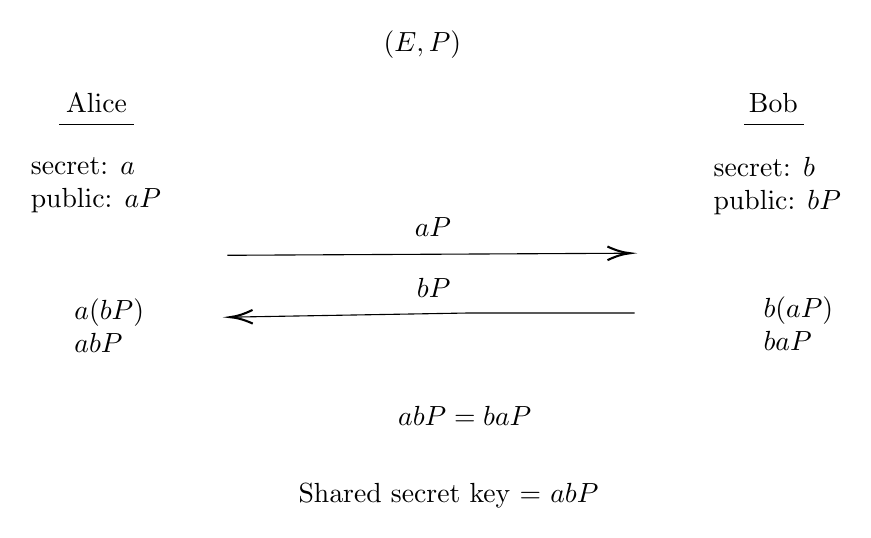
\begin{tikzpicture}[x=0.75pt,y=0.75pt,yscale=-1,xscale=1]
%uncomment if require: \path (0,300); %set diagram left start at 0, and has height of 300

%Straight Lines [id:da1435011466169438] 
\draw    (137,64.4) -- (173,64.4) ;
%Straight Lines [id:da7210376025319416] 
\draw    (467,64.4) -- (496,64.4) ;
%Straight Lines [id:da03246958013588985] 
\draw    (218,127.4) -- (319.21,126.88) -- (410,126.41) ;
\draw [shift={(412,126.4)}, rotate = 179.7] [color={rgb, 255:red, 0; green, 0; blue, 0 }  ][line width=0.75]    (10.93,-3.29) .. controls (6.95,-1.4) and (3.31,-0.3) .. (0,0) .. controls (3.31,0.3) and (6.95,1.4) .. (10.93,3.29)   ;
%Straight Lines [id:da47817176973288045] 
\draw    (414.2,155.2) -- (334.2,155.2) -- (221.2,157.17) ;
\draw [shift={(219.2,157.2)}, rotate = 359] [color={rgb, 255:red, 0; green, 0; blue, 0 }  ][line width=0.75]    (10.93,-3.29) .. controls (6.95,-1.4) and (3.31,-0.3) .. (0,0) .. controls (3.31,0.3) and (6.95,1.4) .. (10.93,3.29)   ;

% Text Node
\draw (139,48) node [anchor=north west][inner sep=0.75pt]   [align=left] {Alice};
% Text Node
\draw (468,48) node [anchor=north west][inner sep=0.75pt]   [align=left] {Bob};
% Text Node
\draw (122,79) node [anchor=north west][inner sep=0.75pt]   [align=left] {secret: \(a\)\\public: \(aP\)};
% Text Node
\draw (292,18) node [anchor=north west][inner sep=0.75pt]   [align=left] {\((E, P)\)};
% Text Node
\draw (451,79) node [anchor=north west][inner sep=0.75pt]   [align=left] {secret: \(b\)\\public: \(bP\)};
% Text Node
\draw (307,108) node [anchor=north west][inner sep=0.75pt]   [align=left] {\(aP\)};
% Text Node
\draw (308,137) node [anchor=north west][inner sep=0.75pt]   [align=left] {\(bP\)};
% Text Node
\draw (143,147) node [anchor=north west][inner sep=0.75pt]   [align=left] {\(a(bP)\)\\\(abP\)};
% Text Node
\draw (475,146) node [anchor=north west][inner sep=0.75pt]   [align=left] {\(b(aP)\)\\\(baP\)};
% Text Node
\draw (299,199) node [anchor=north west][inner sep=0.75pt]   [align=left] {\(abP=baP\)};
% Text Node
\draw (251,236) node [anchor=north west][inner sep=0.75pt]   [align=left] {Shared secret key = \(abP\)};

\end{tikzpicture}
\end{center}

In the above scenario, \( E \) and \( P \) were public while \( a \) and \( b \) were secret. Since \( a \), \( b \), \( P \) are all discrete, we can find \( aP \) (a times \( P \)), \( bP \) (b times \( P \)), and so on. Since they are discrete, \( abP \) and \( baP \) are the same. Since both Alice and Bob finally reached the same point on the curve, they have successfully exchanged messages.\\
\textbf{Note:} Security of ECDH depends on the fact that finding \( xP \) from \( P \) is computationally difficult. This hard problem is known as the \textbf{Discrete Log Problem on EC}.


\section*{RSA Signature}

RSA Signature Encryption/Decryption:
\[
\text{Encryption: } c = x^e \mod n, \quad \text{Decryption: } x = c^d \mod n
\]
\[
\text{Signature: } s = x^d \mod n, \quad \text{Verification: } x = s^e \mod n
\]


\section*{Elliptic Curve Digital Signature Algorithm (ECDSA)}

In ECDSA, a public key $P$ corresponds to a secret key $a$, where the public key is represented as $aP$.

\subsection*{Properties of ECDSA}
\begin{itemize}
    \item ECDSA relies on a large prime number $n$, ensuring that $nG = 0$ on the elliptic curve, where $G$ is the base point, and $(n-1)G \oplus G = nG$.
\end{itemize}

\subsection*{Signature Generation Process}
\begin{enumerate}
    \item Compute the hash $e$ of the message $m$.
    \item Select the leftmost $L_n$ bits of $e$, where $L_n$ is the bit length of $n$.
    \item Choose a random integer $k$ from the range $[1, n-1]$.
    \item Generate a key pair $(x_1, y_1)$.
    \item Calculate $r = x_1 \mod n$. If $r = 0$, repeat step 1.
    \item Calculate $s = k^{-1}(z + r \cdot d_A) \mod n$, where $d_A$ is the secret key. If $s = 0$, repeat step 1.
    \item The signature on message $m$ is $(r, s)$.
\end{enumerate}

\subsection*{Verification Process by Bob}
\begin{enumerate}
    \item Ensure that the public key $Q_A$ is not equal to $0$.
    \item Verify if $Q_A$ lies on the elliptic curve.
    \item Verify if $n \cdot Q_A = n \cdot d_A \cdot a$, where $Q_A = d_A \cdot G$.
\end{enumerate}

\subsection*{Additional Verification Steps}
\begin{enumerate}
    \item Check if $r$ and $s$ are within the range $[1, n-1]$.
    \item Compute $e$ by hashing the message $m$.
    \item Select the leftmost bits of $e$.
    \item Compute $u_1 = z \cdot s^{-1} \mod n$ and $u_2 = r \cdot s^{-1} \mod n$.
    \item Calculate the point $(x_2, y_2) = u_1 \cdot a + u_2 \cdot Q_A$. If $(x_2, y_2) = 0$, the signature is invalid.
    \item Verify if $r \equiv x_2 \mod n$. If this condition holds, the signature is valid; otherwise, it is invalid.
    \item Recompute $e$ using $u_1 \cdot a + u_2 \cdot Q_A$. If the result matches the original hash $e$, the verification is successful.
\end{enumerate}


\end{document}